\begin{frame}{presenter}
  \begin{figure}
    \centering
    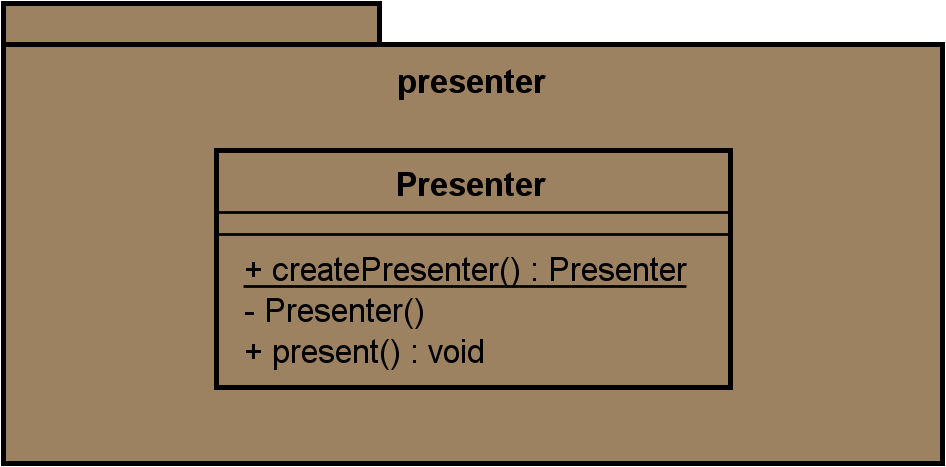
\includegraphics[width=0.4\textwidth]{./images/presenter.png}
  \end{figure}
  \begin{itemize}[<+->]
    \item Aufgaben
      \begin{itemize}
        \item Wichtig bei Programmstart, Aufruf in der main Methode
        \item Instanziieren und Initialisieren der Programmelemente
        \item Aufrufen der Services
        \item Übergeben der Abhängigkeiten und Bestimmung der Nutzerrelationen
      \end{itemize}
      \item Entwurfsentscheidungen
        \begin{itemize}
          \item Erster Teil der Variation des Controllers
          \item Entkopplung von Initialisierung und dauerhaften Programmabläufen
          \item Leicht änderbarer Programmaufbau
        \end{itemize}
  \end{itemize}
\end{frame}
